\section{Appendix}

\subsection{Extensions}
\subsubsection{MIN and MAX}
\minfunc and \maxfunc fall into their own category since this is a canonical case where bootstrap fails.
We devise an estimation procedure that corrects these queries.
However, we can only achieve bound that has a slightly different interpretation than the confidence intervals seen before.
We can calculate the probability that a larger (or smaller) element exists in the unsampled view.
%Refer to the extended technical report for the details on \minfunc and \maxfunc \cite{technicalReport}.

We devise the following correction estimate for \maxfunc: (1) For all rows in both $S$ and $S'$, calculate the row-by-row difference, (2) let $c$ be the max difference, and (3) add $c$ to the max of the stale view.

We can give weak bounds on the results using Cantelli's Inequality.
If $X$ is a random variable with mean $\mu_x$ and variance $var(X)$, then the probability that $X$ is larger than a constant $\epsilon$ 
\[
\mathbb{P}(X \ge \epsilon + \mu_x ) \le \frac{var(X)}{var(X) + \epsilon^2}
\]
Therefore, if we set $\epsilon$ to be the difference between max value estimate and the average value, we can calculate the probability that we will see a higher value. 

The same estimator can be modified for \minfunc, with a corresponding bound:
\[
\mathbb{P}(X \le \mu_x - a )) \le \frac{var(x)}{var(x) + a^2}
\]
This bound has a slightly different interpretation than the confidence intervals seen before.
This gives the probability that a larger (or smaller) element exists in the unsampled view.


\vspace{-.25em}
\subsubsection{Select Queries}
In \svc, we also explore how to extend this correction procedure to Select queries.
Suppose, we have a Select query with a predicate:
\begin{lstlisting} [mathescape]
SELECT $*$ FROM View WHERE Condition(A);
\end{lstlisting}

We first run the Select query on the stale view, and this returns a set of rows.
This result has three types of data error: rows that are missing, rows that are falsely included, and rows whose values are incorrect.

As in the \sumfunc, \countfunc, and \avgfunc query case, we can apply the query to the sample of the up-to-date view.
From this sample, using our lineage defined earlier, we can quickly identify which rows were added, updated, and deleted.
For the updated rows in the sample, we overwrite the out-of-date rows in the stale query result.
For the new rows, we take a union of the sampled selection and the updated stale selection.
For the missing rows, we remove them from the stale selection.
To quantify the approximation error, we can rewrite the Select query as \countfunc to get an estimate of number of rows that were updated, added, or deleted (thus three ``confidence'' intervals).

\subsection{Additional Experiments}

\subsubsection{Aggregate View}
\label{exp-datacube}

\begin{figure}[t]
\centering
 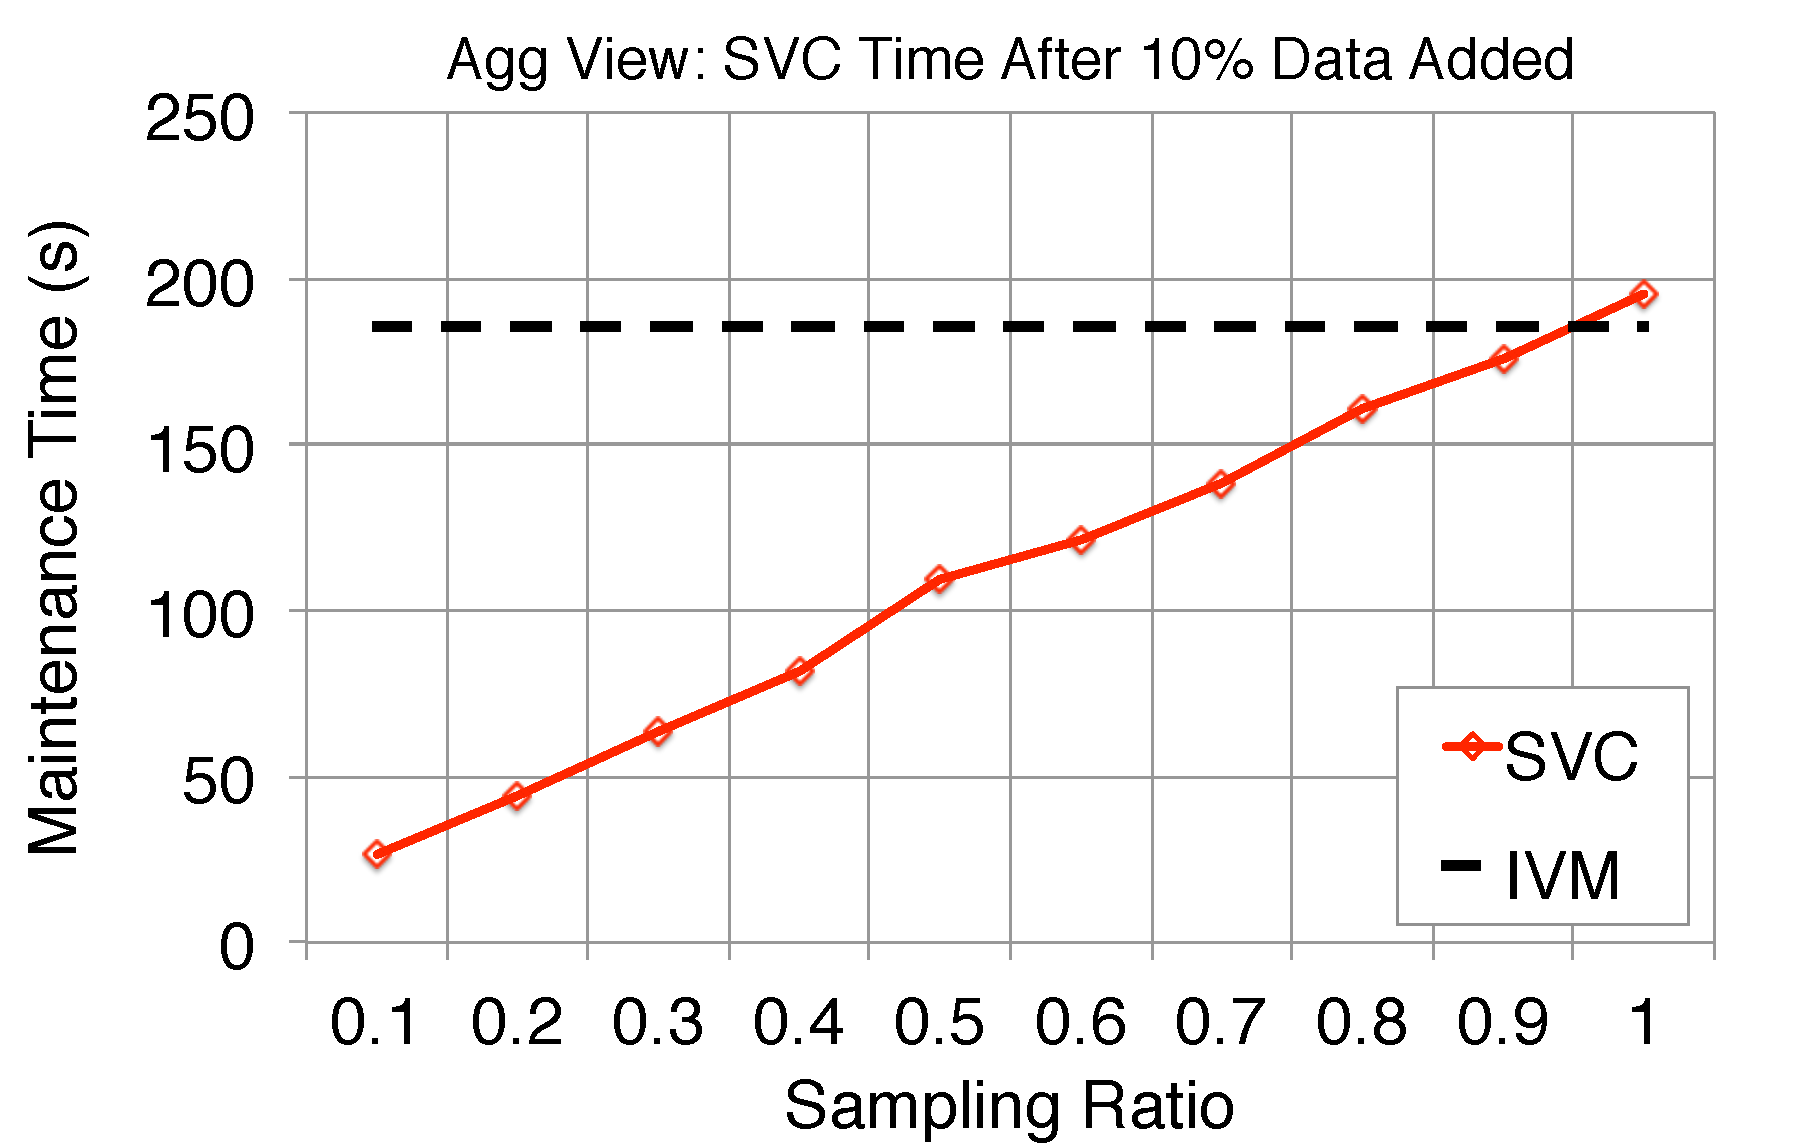
\includegraphics[scale=0.15]{exp/msdc_1.pdf}
 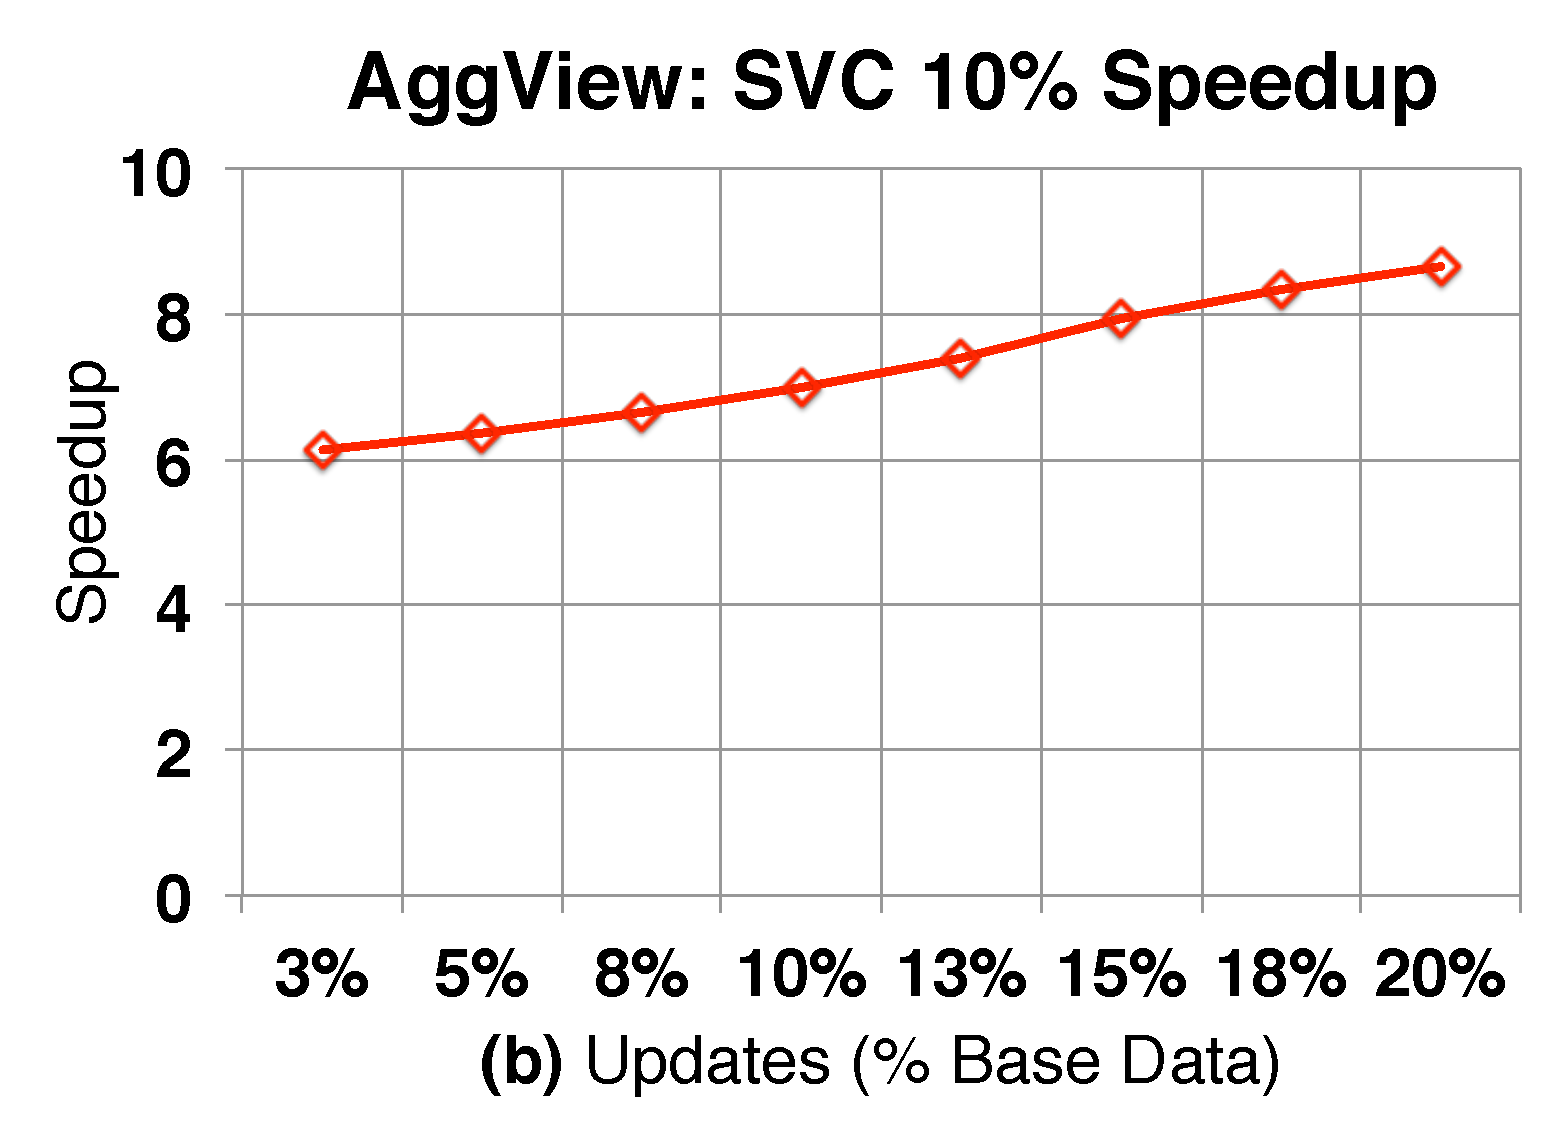
\includegraphics[scale=0.15]{exp/msdc_2.pdf}
  %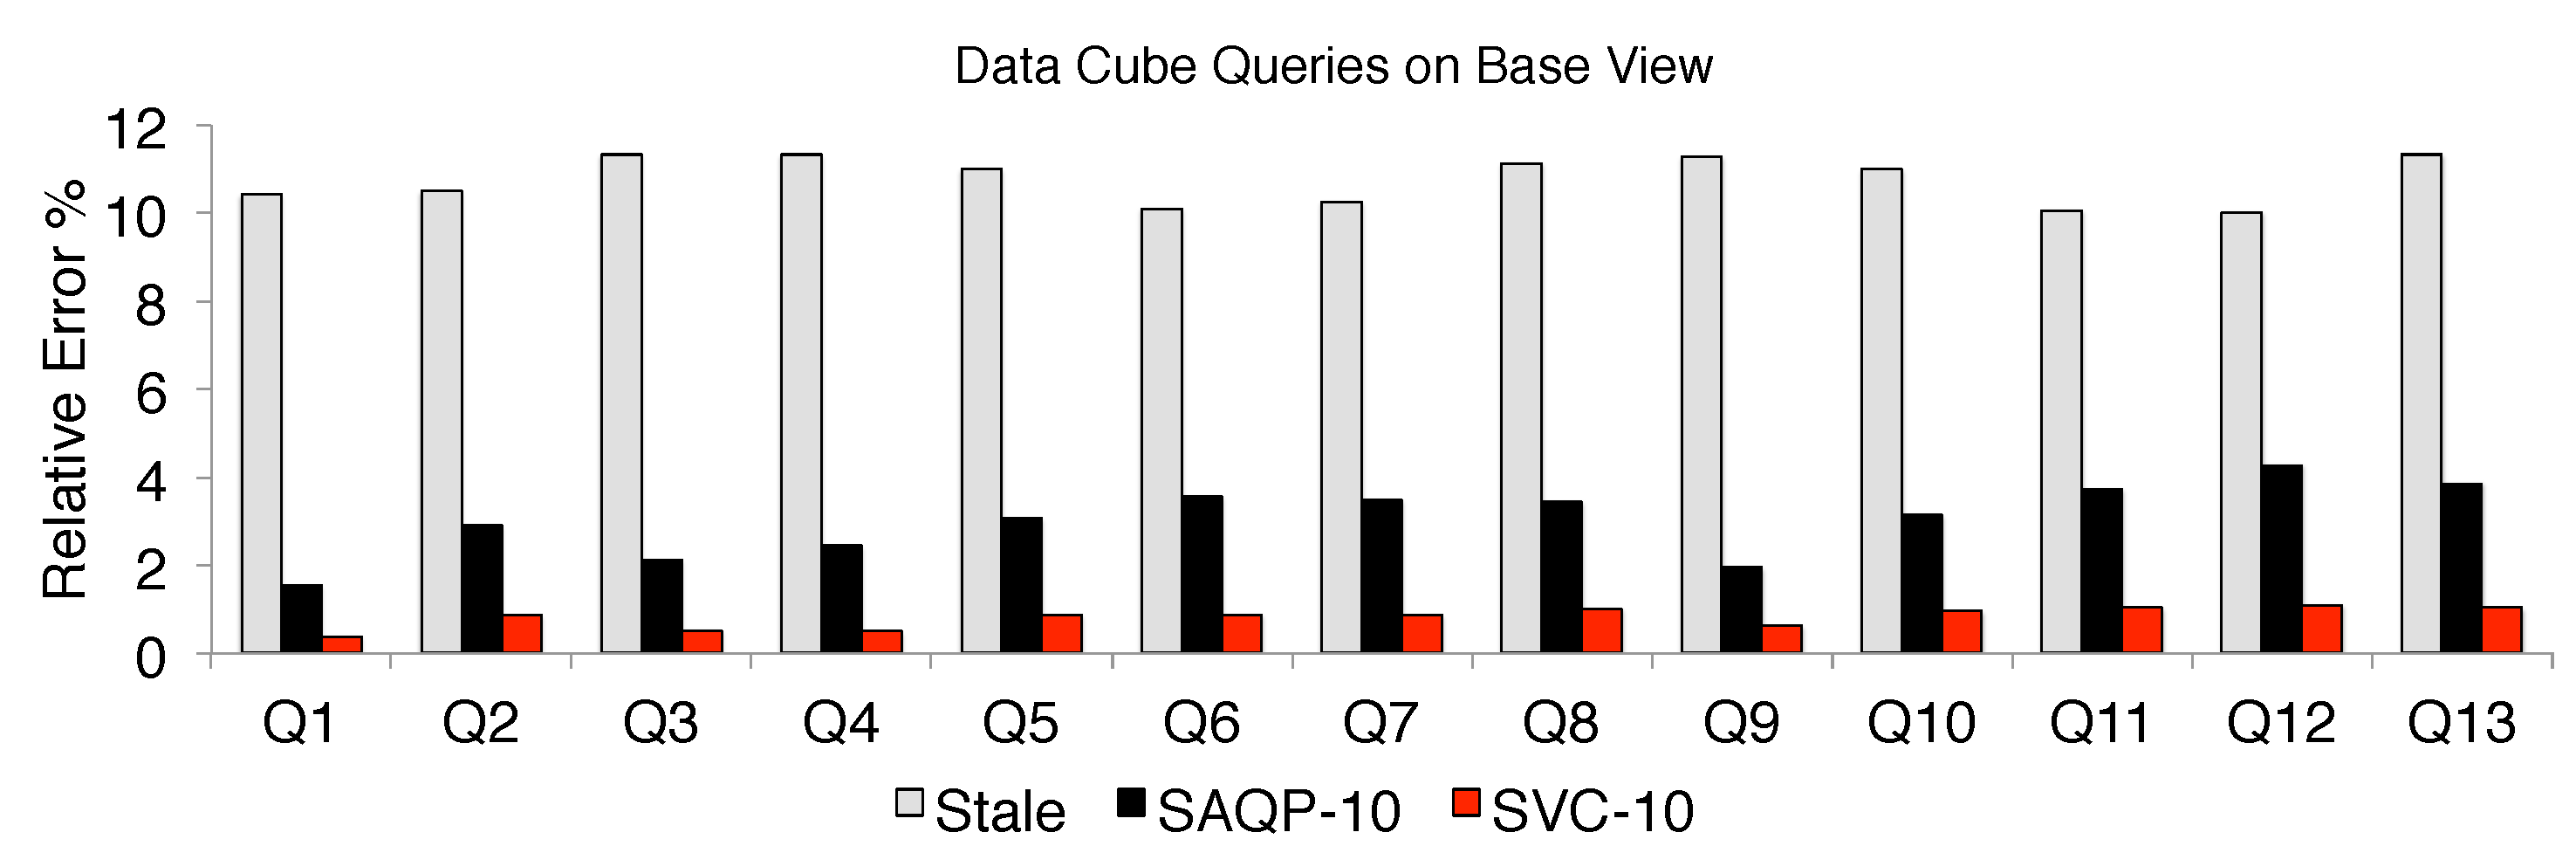
\includegraphics[scale=0.17]{exp/msdc_3.pdf}
   \caption{(a) In the aggregate view case, sampling can save significant maintenance time. (b) As the update size grows SVC tends towards an ideal speedup of 10x.\label{exp2-acc-sample}}
\end{figure}


\begin{figure}[t]
\centering
 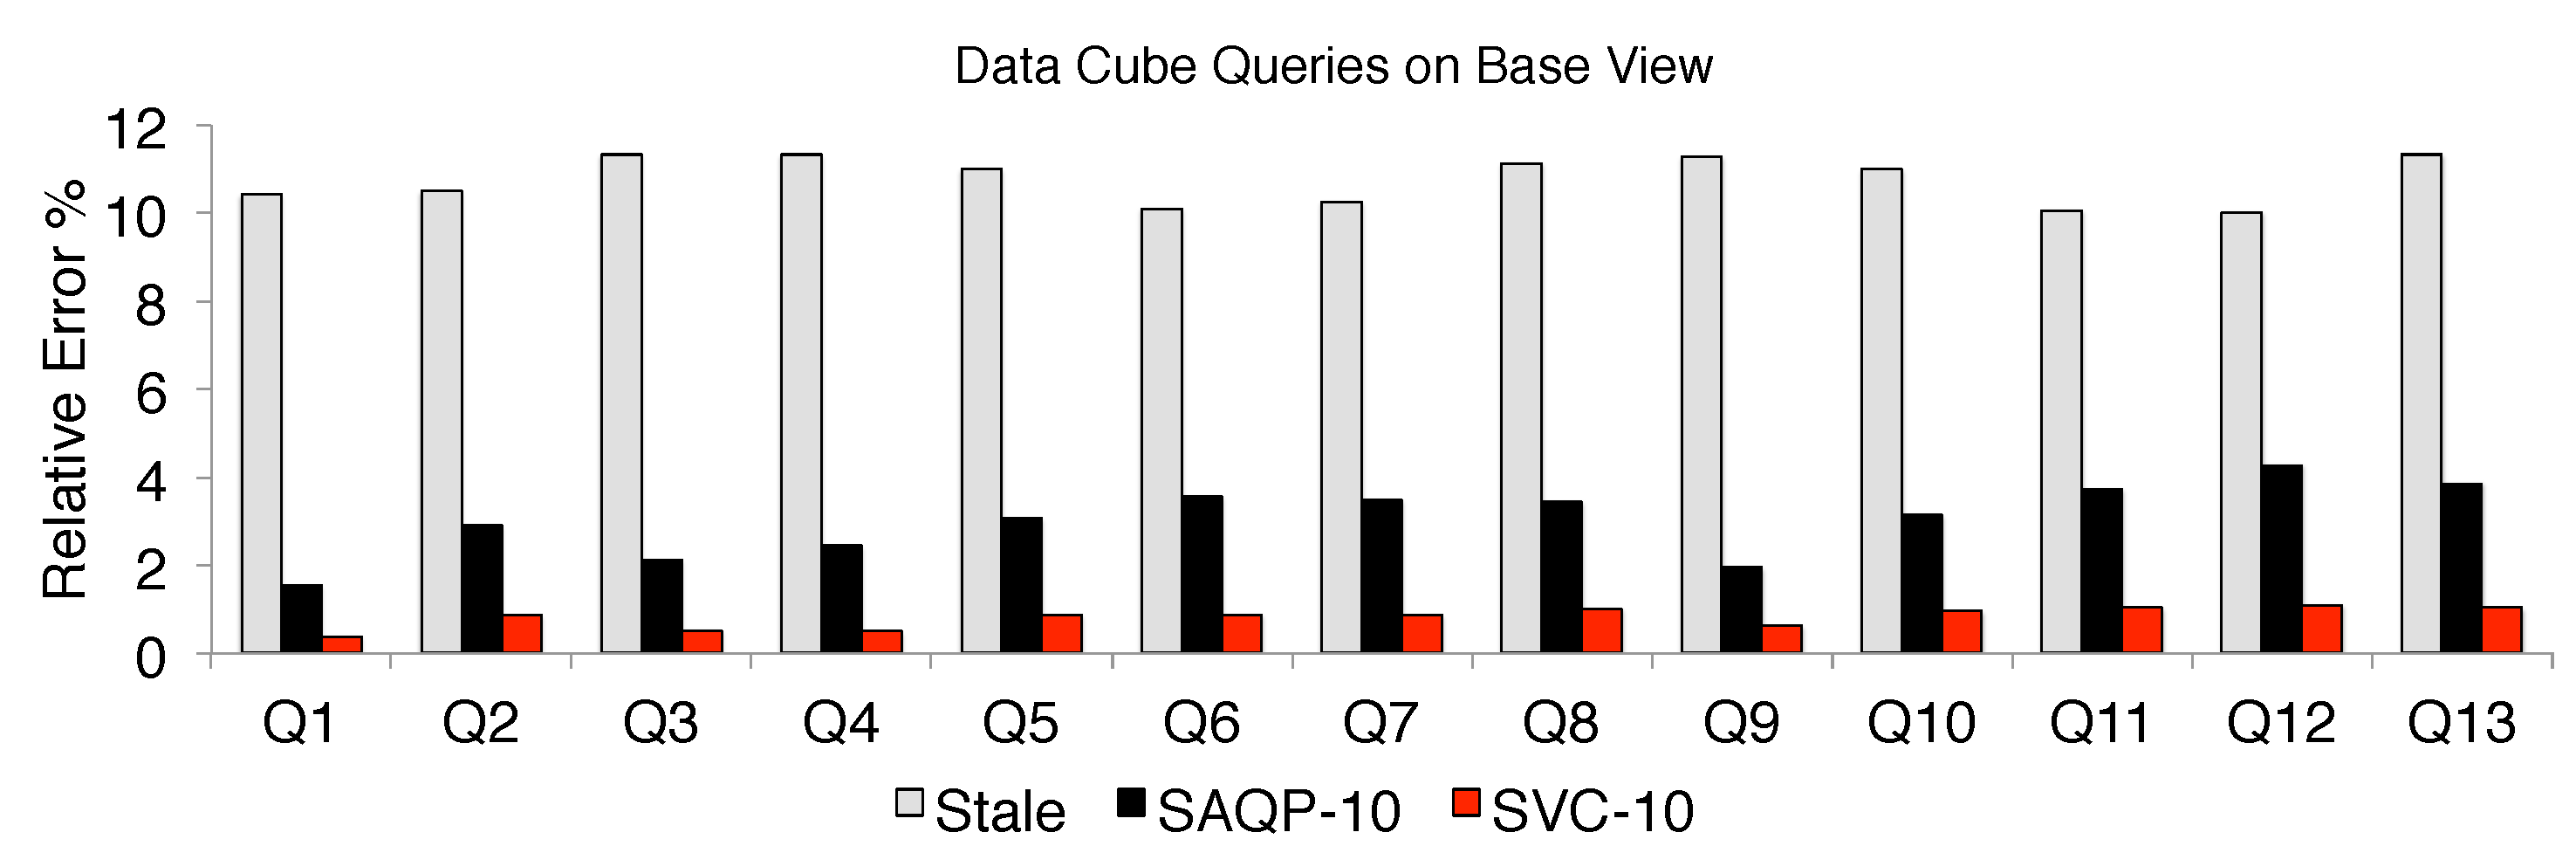
\includegraphics[scale=0.17]{exp/msdc_3.pdf}
   \caption{We measure the accuracy of each of the roll-up aggregate queries on this view. For a 10\% sample size and 10\% update size, we find that SVC+Corr is more accurate than SVC+AQP and No Maintenance.\label{exp2-acc-sample2}}
\end{figure}



\begin{figure}[t]
\centering
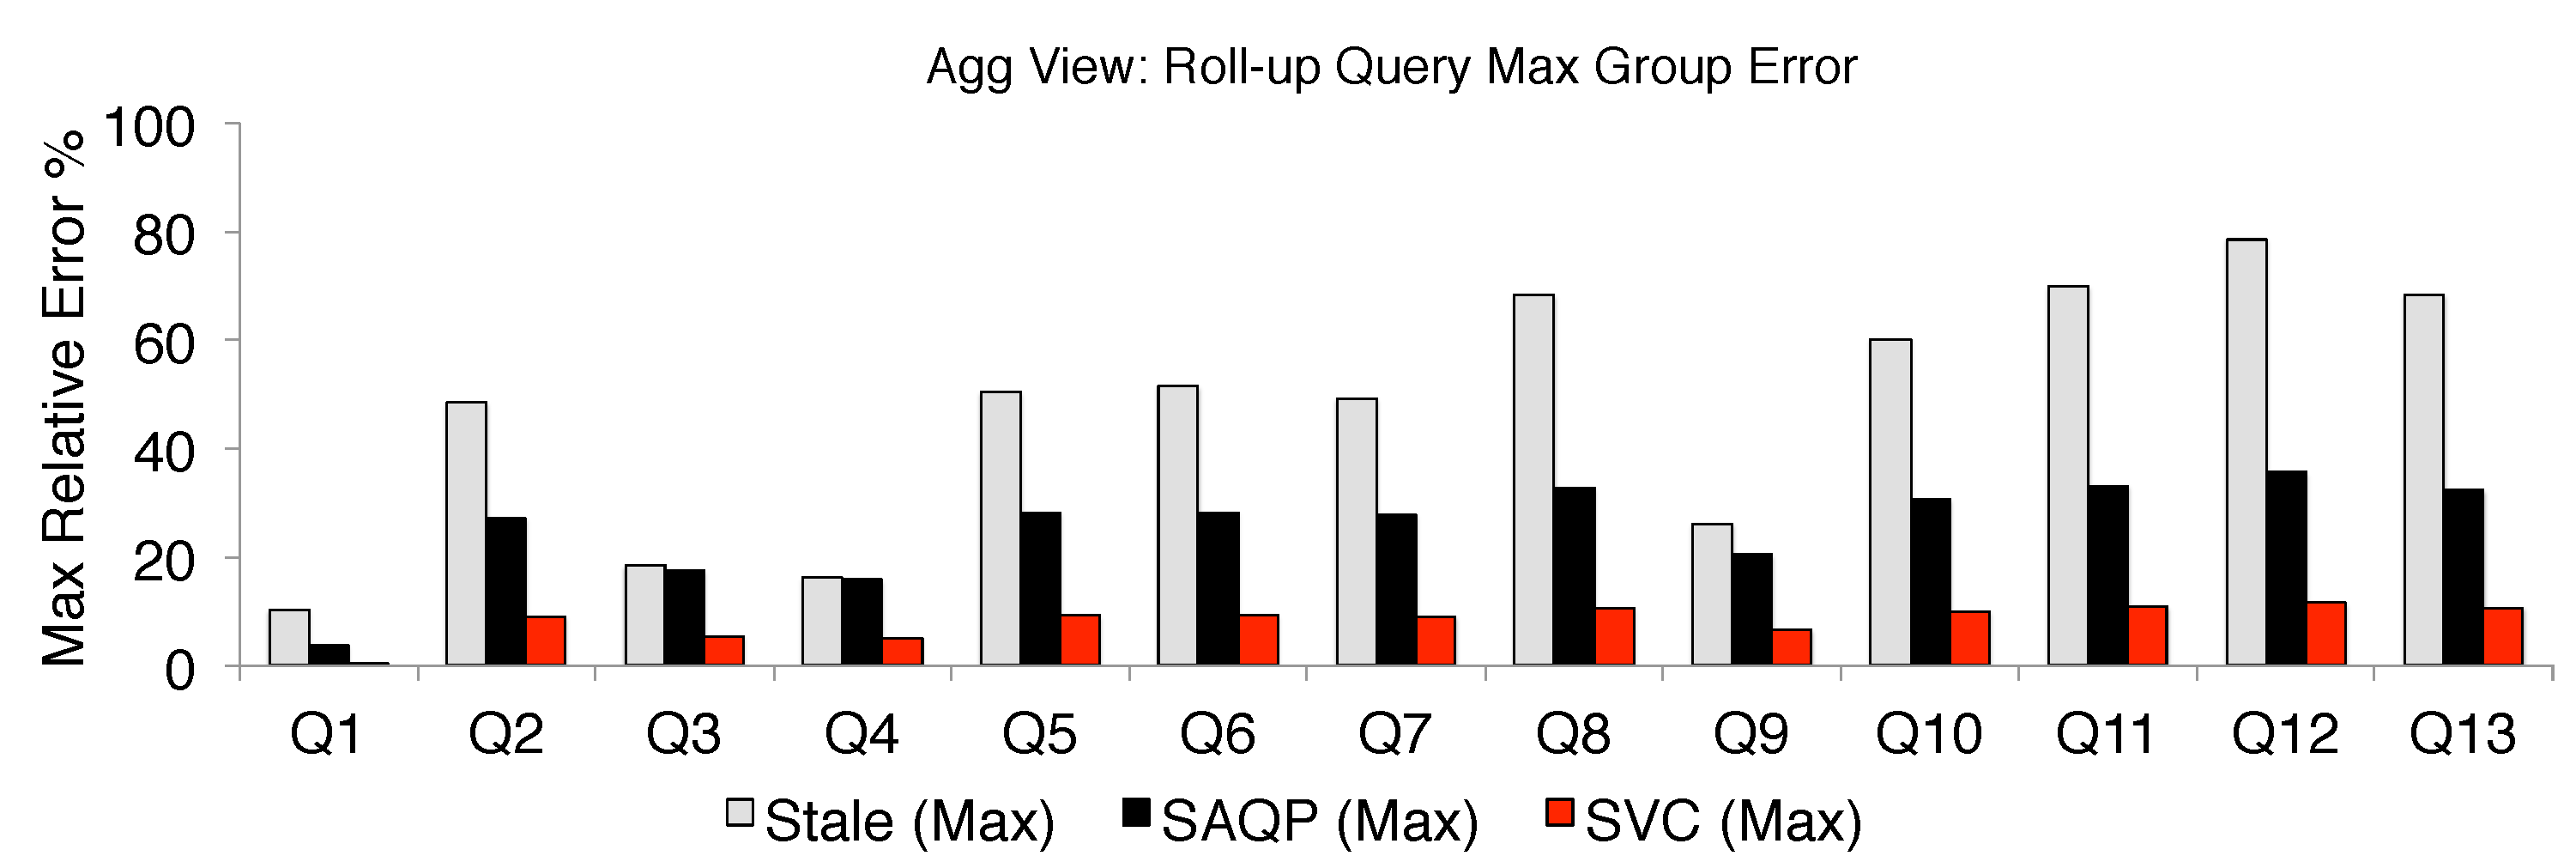
\includegraphics[scale=0.17]{exp/msdc_4.pdf}
   \caption{For 1GB of updates, we plot the max error as opposed to the median error in the previous experiments. Even though updates are 10\% of the dataset size, some queries are nearly 80\% incorrect. SVC helps significantly mitigate this error. \label{exp2-max}}
\end{figure}

\begin{figure}[t]
\centering
  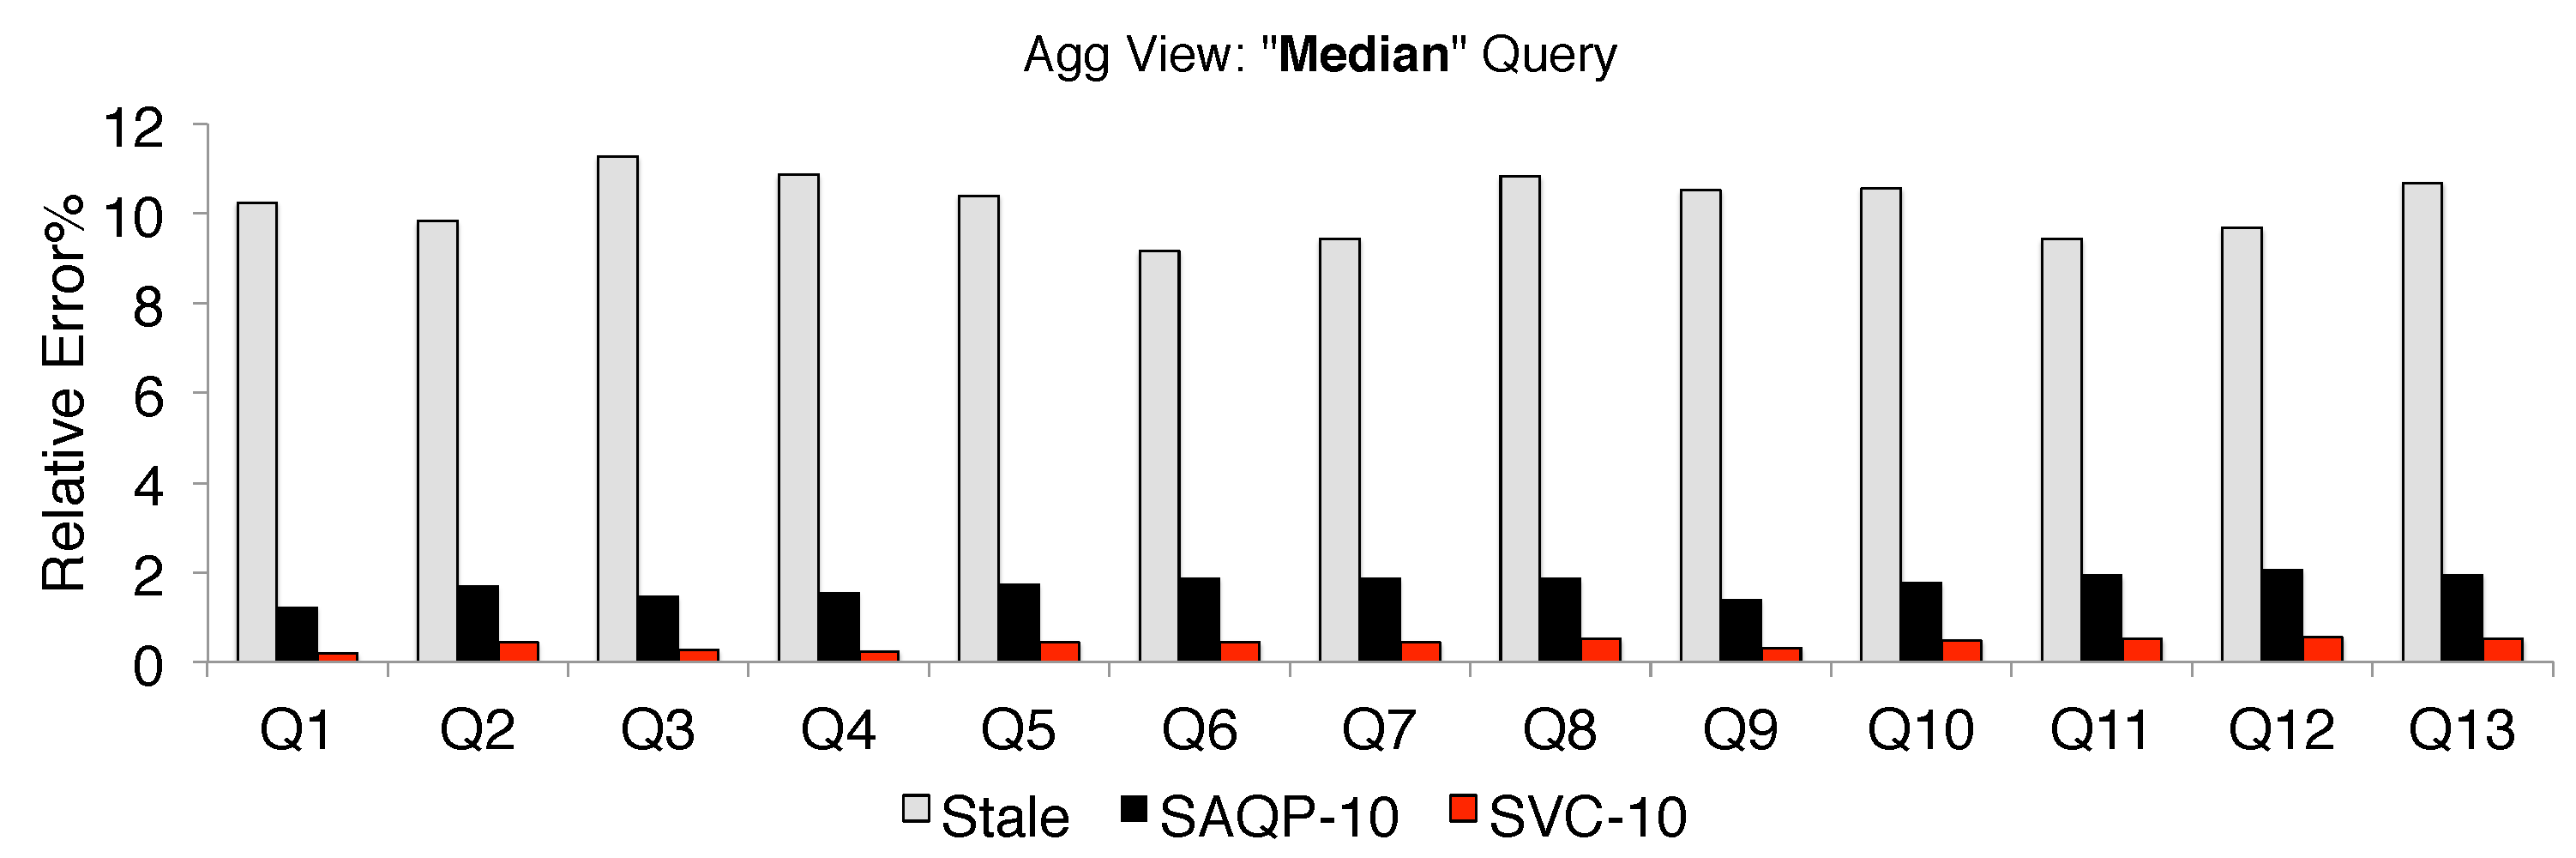
\includegraphics[scale=0.17]{exp/msdc_5.pdf}
  %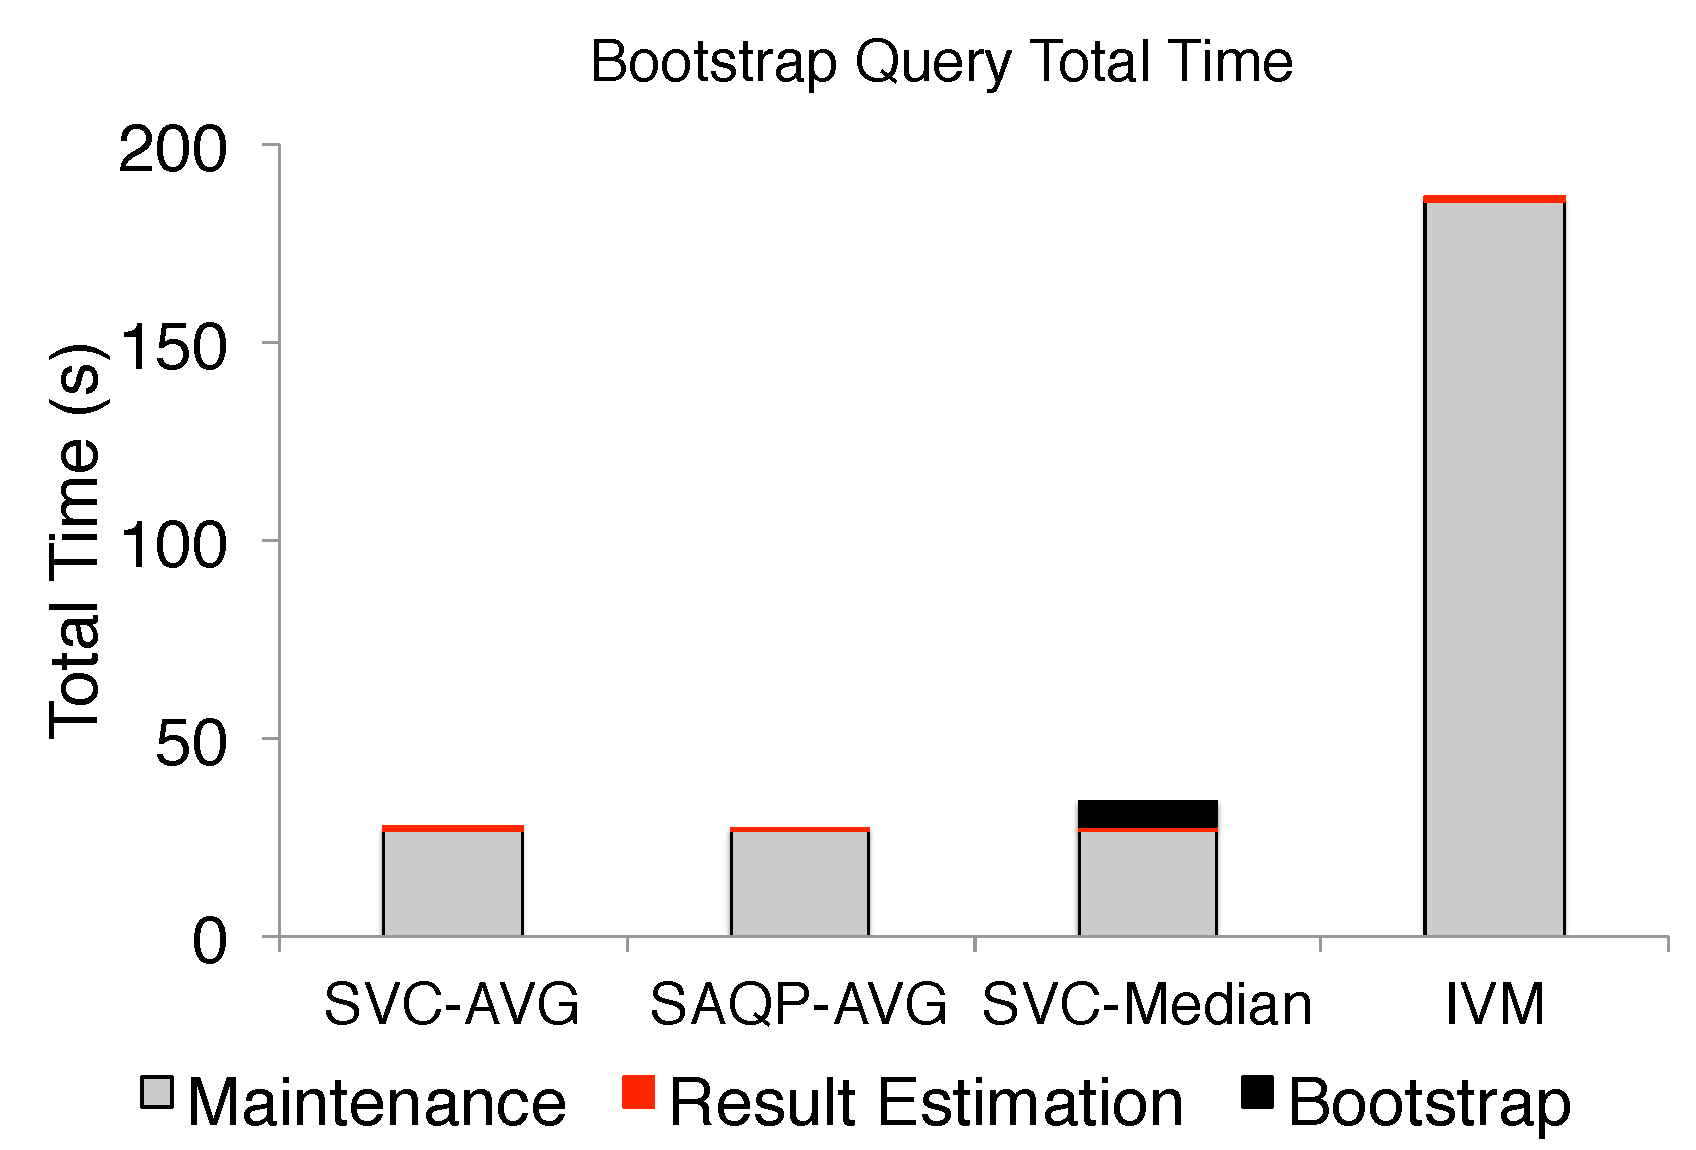
\includegraphics[scale=0.20]{exp/msdc_6.pdf}
 \caption{We run the same experiment but replace the \sumfunc query with a median query. We find that similarly SVC is more accurate.\label{exp2-median} }
\end{figure}

In our next experiment, we evaluate an aggregate view use case similar to a data cube.
We generate a 10GB base TPCD dataset with skew $z=1$, and derive the base cube as a materialized view from this dataset.
We add 1GB of updates and apply SVC to estimate the results of all of the ``roll-up" dimensions.

\textbf{Performance: }
We observed the same trade-off as the previous experiment where sampling significantly reduces the maintenance time (Figure \ref{exp2-acc-sample}(a)).
It takes 186 seconds to maintain the entire view, but a 10\% sample can be maintained in 26 seconds.
As before, we fix the sample size at 10\% and vary the update size.
We similarly observe that SVC becomes more efficient as the update size grows (Figure \ref{exp2-acc-sample}(b)), and at an update size of 20\%  the speedup is 8.7x.

\textbf{Accuracy: }
In Figure \ref{exp2-acc-sample2}, we measure the accuracy of each of the ``roll-up" aggregate queries on this view.
That is, we take each dimension and aggregate over the dimension.
We fix the sample size at 10\% and the update size at 10\%.
On average SVC+Corr is 12.9x more accurate than the stale baseline and 3.6x more accurate than SVC+AQP (Figure \ref{exp2-acc-sample}(c)). 

Since the data cubing operation is primarily constructed by group-by aggregates, we can also measure the max error for each of the aggregates.
We see that while the median staleness is close to 10\%, for some queries some of the group aggregates have nearly 80\% error (Figure \ref{exp2-max}).
SVC greatly mitigates this error to less than 12\% for all queries.

\textbf{Other Queries: }
Finally, we also use the data cube to illustrate how SVC can support a broader range of queries outside of \sumfunc, \countfunc, and \avgfunc.
We change all of the roll-up queries to use the \textbf{median} function (Figure \ref{exp2-median}).
First, both SVC+Corr and SVC+AQP are more accurate as estimating the median than they were for estimating sums. 
This is because the median is less sensitive to variance in the data.

\subsubsection{Mini-batch Experiments}
\begin{figure}[t]
\centering
 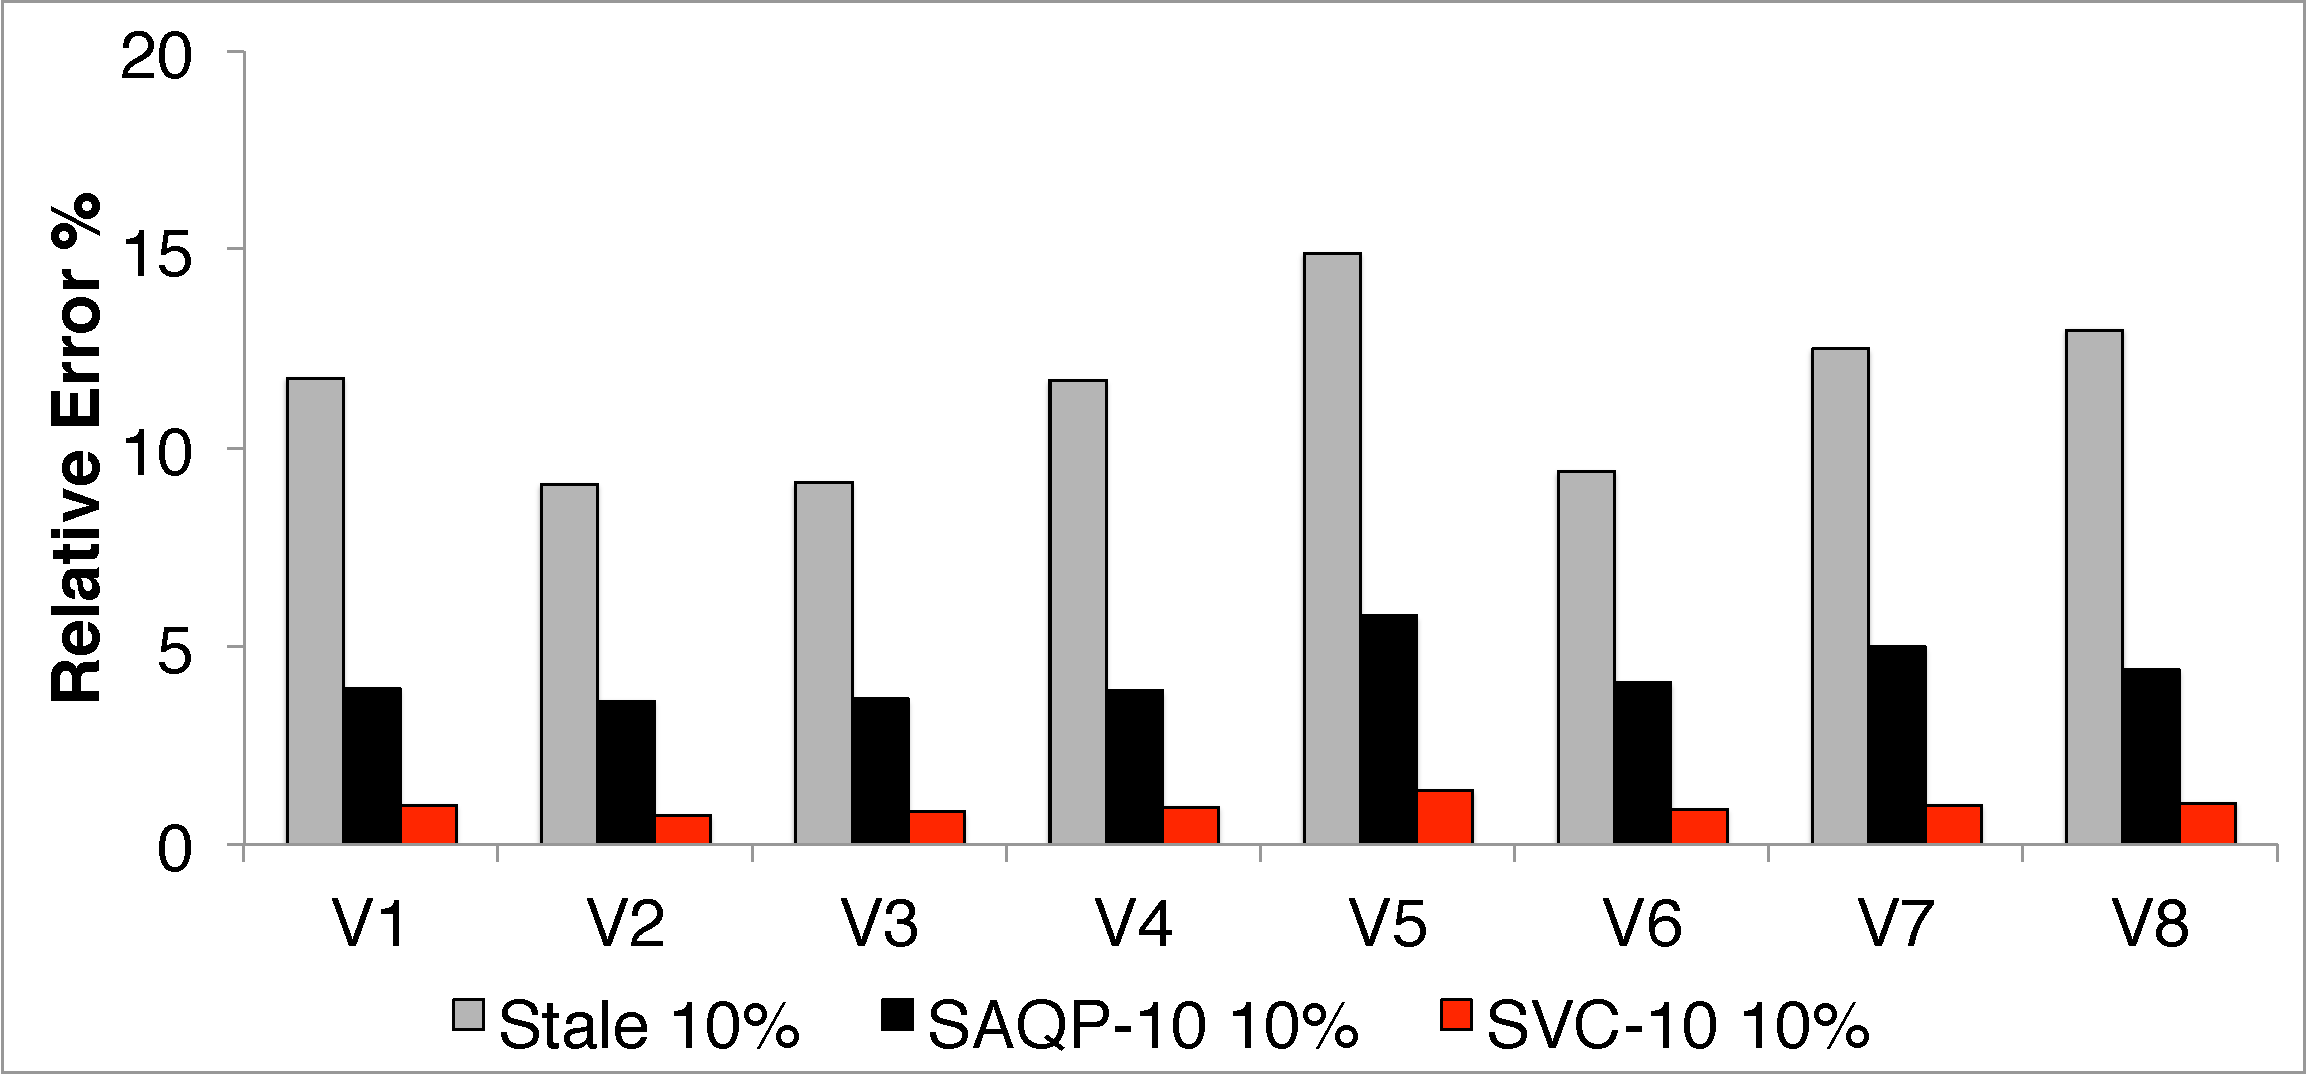
\includegraphics[scale=0.14]{exp/con_1.pdf}
 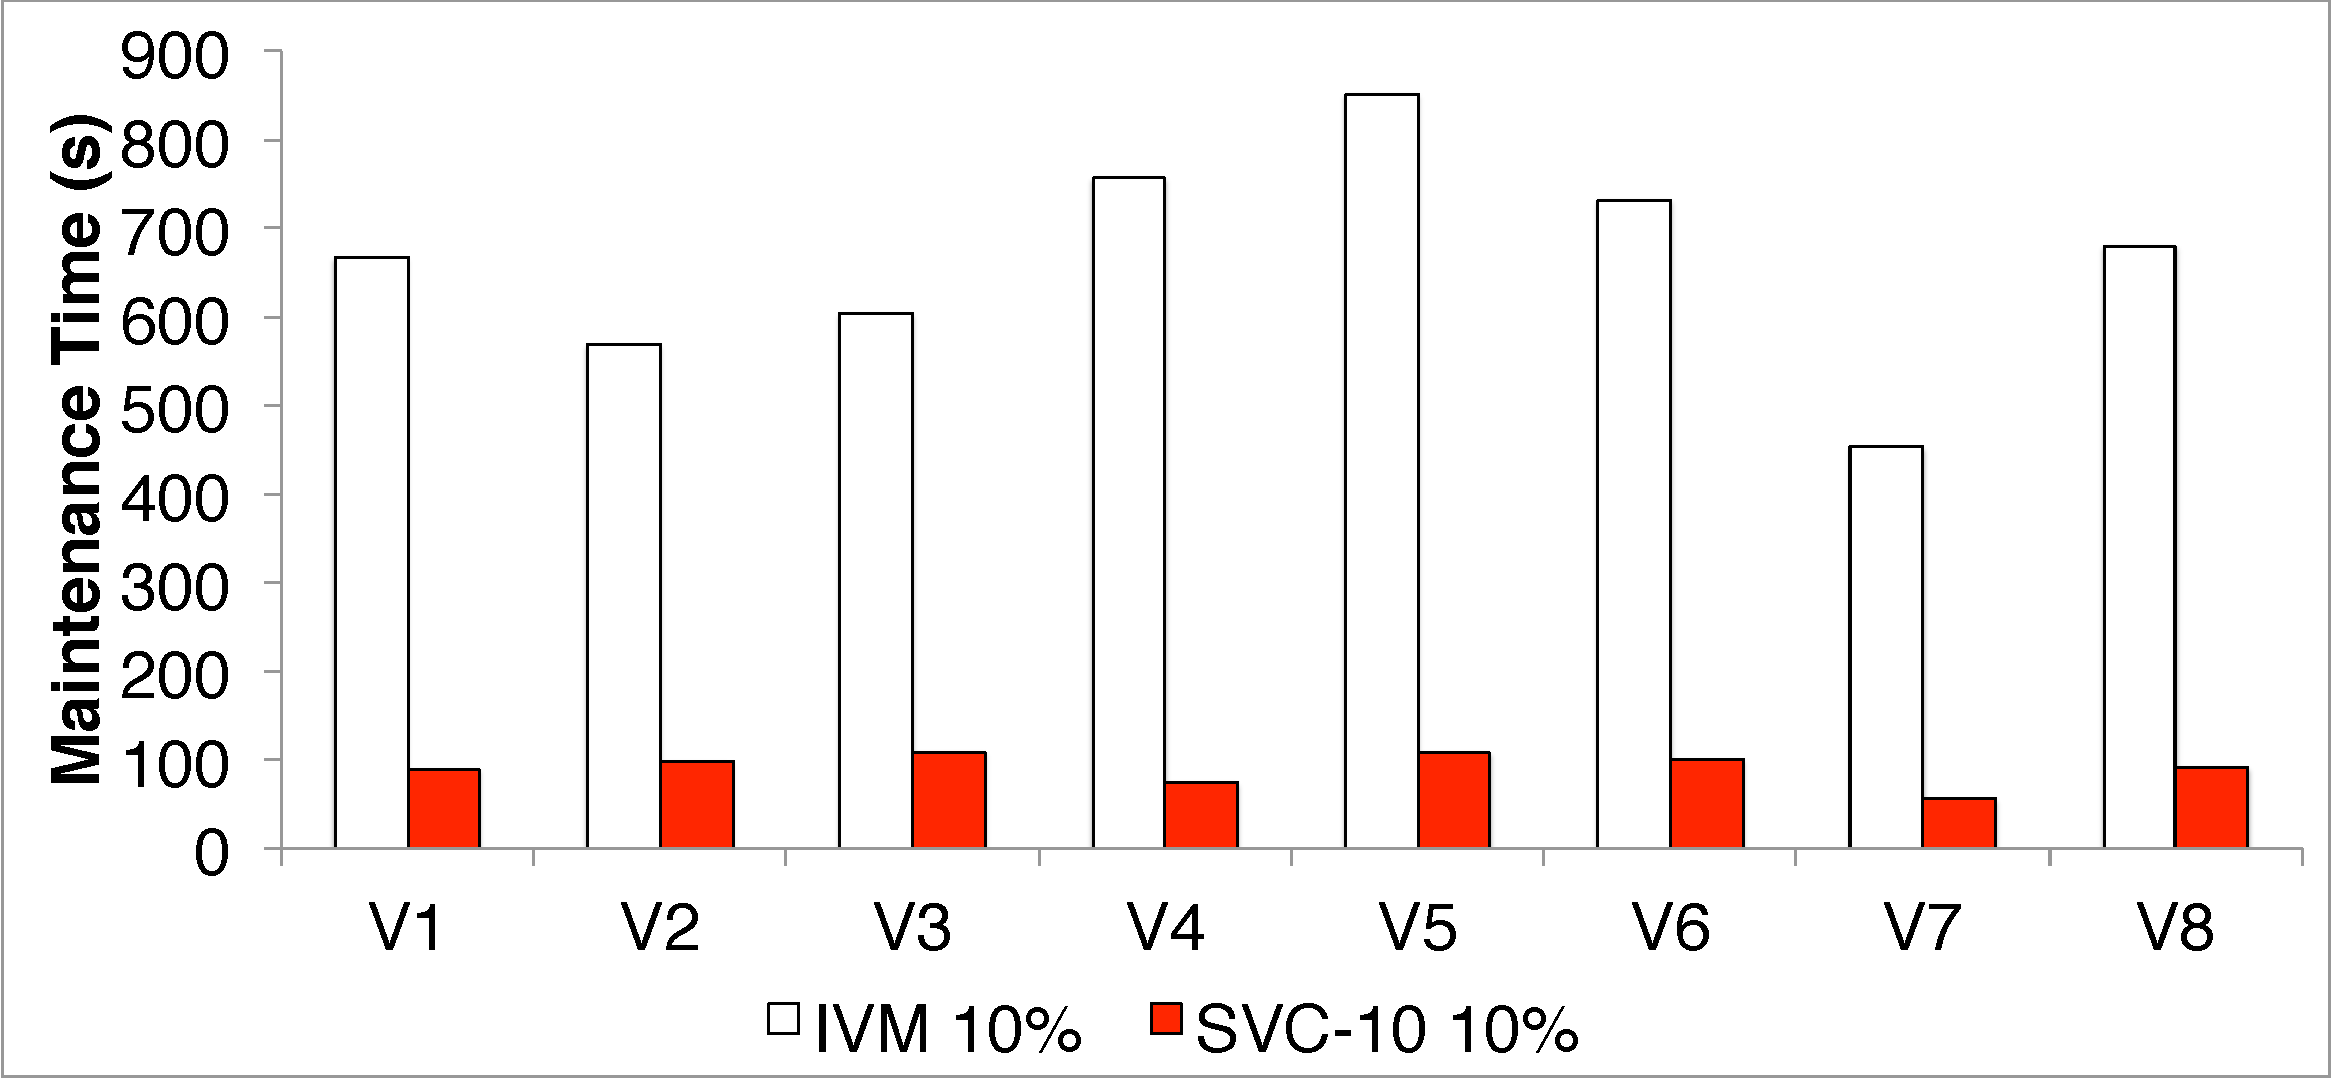
\includegraphics[scale=0.14]{exp/con_2.pdf}
 \caption{(a) Spark RDDs are most efficient when updated in batches. As batch sizes increase the system throughput increases. (b) When running multiple threads, the throughput reduces. However, larger batches are less affected by this reduction. \label{conv-2}}
\end{figure}

We devised an end-to-end experiment simulating a real integration with periodic maintenance.
However, unlike the MySQL case, Apache Spark does not support selective updates and insertions as the ``views" are immutable.
A further point is that the immutability of these views and Spark's fault-tolerance requires that the ``views" are maintained synchronously.
Thus, to avoid these significant overheads, we have to update these views in batches.
Spark does have a streaming variant \cite{zaharia2012discretized}, however, this does not support the complex SQL derived materialized views used in this paper, and still relies on mini-batch updates.

SVC and IVM will run in separate threads each with their own RDD materialized view.
In this application, both SVC and IVM maintain respective their RDDs with batch updates.
In this model, there are a lot of different parameters: batch size for periodic maintenance, batch size for SVC, sampling ratio for SVC, and the fact that concurrent threads may reduce overall throughput.
Our goal is to fix the throughput of the cluster, and then measure whether SVC+IVM or IVM alone leads to more accurate query answers.

\textbf{Batch sizes:} In Spark, larger batch sizes amortize overheads better.
In Figure \ref{conv-2}(a), we show a trade-off between batch size and throughput of Spark for V2 and V5.
Throughputs for small batches are nearly 10x smaller than the throughputs for the larger batches. 

\textbf{Concurrent SVC and IVM:} Next, we measure the reduction in throughput when running multiple threads.
We run SVC-10 in loop in one thread and IVM in another.
We measure the reduction in throughput for the cluster from the previous batch size experiment.
In Figure \ref{conv-2}(b), we plot the throughput against batch size when two maintenance threads are running.
While for small batch sizes the throughput of the cluster is reduced by nearly a factor of 2, for larger sizes the reduction is
smaller.
As we found in later experiments (Figure \ref{conv-5}), larger batch sizes are more amenable to parallel computation since there was more idle CPU time.

\textbf{Choosing a Batch Size:}
The results in Figure \ref{conv-2}(a) and Figure \ref{conv-2}(b) show that larger batch sizes are more efficient, however, larger batch sizes also lead to more staleness.
Combining the results in Figure \ref{conv-2}(a) and Figure \ref{conv-2}(b), for both SVC+IVM and IVM, we get cluster throughput as a function of batch size.
For a fixed throughput, we want to find the smallest batch size that achieves that throughput for both.
For V2, we fixed this at 700,000 records/sec and for V5 this was 500,000 records/sec.
For IVM alone the smallest batch size that met this throughput demand was 40GB for both V2 and V5.
And for SVC+IVM, the smallest batch size was 80GB for V2 and 100GB for V5. 
When running periodic maintenance alone view updates can be more frequent, and when run in conjunction with SVC it is less frequent. 

We run both of these approaches in a continuous loop, SVC+IVM and IVM, and measure their maximal error during a maintenance period.
There is further a trade-off with the sampling ratio, larger samples give more accurate estimates however between SVC batches they go stale.
We quantify the error in these approaches with the max error; that is the maximum error in a maintenance period (Figure \ref{conv-4}).
These competing objective lead to an optimal sampling ratio of 3\% for V2 and 6\% for V5.
At this sampling point, we find that applying SVC gives results 2.8x more accurate for V2 and 2x more accurate for V5.

\begin{figure}[t]
\centering
 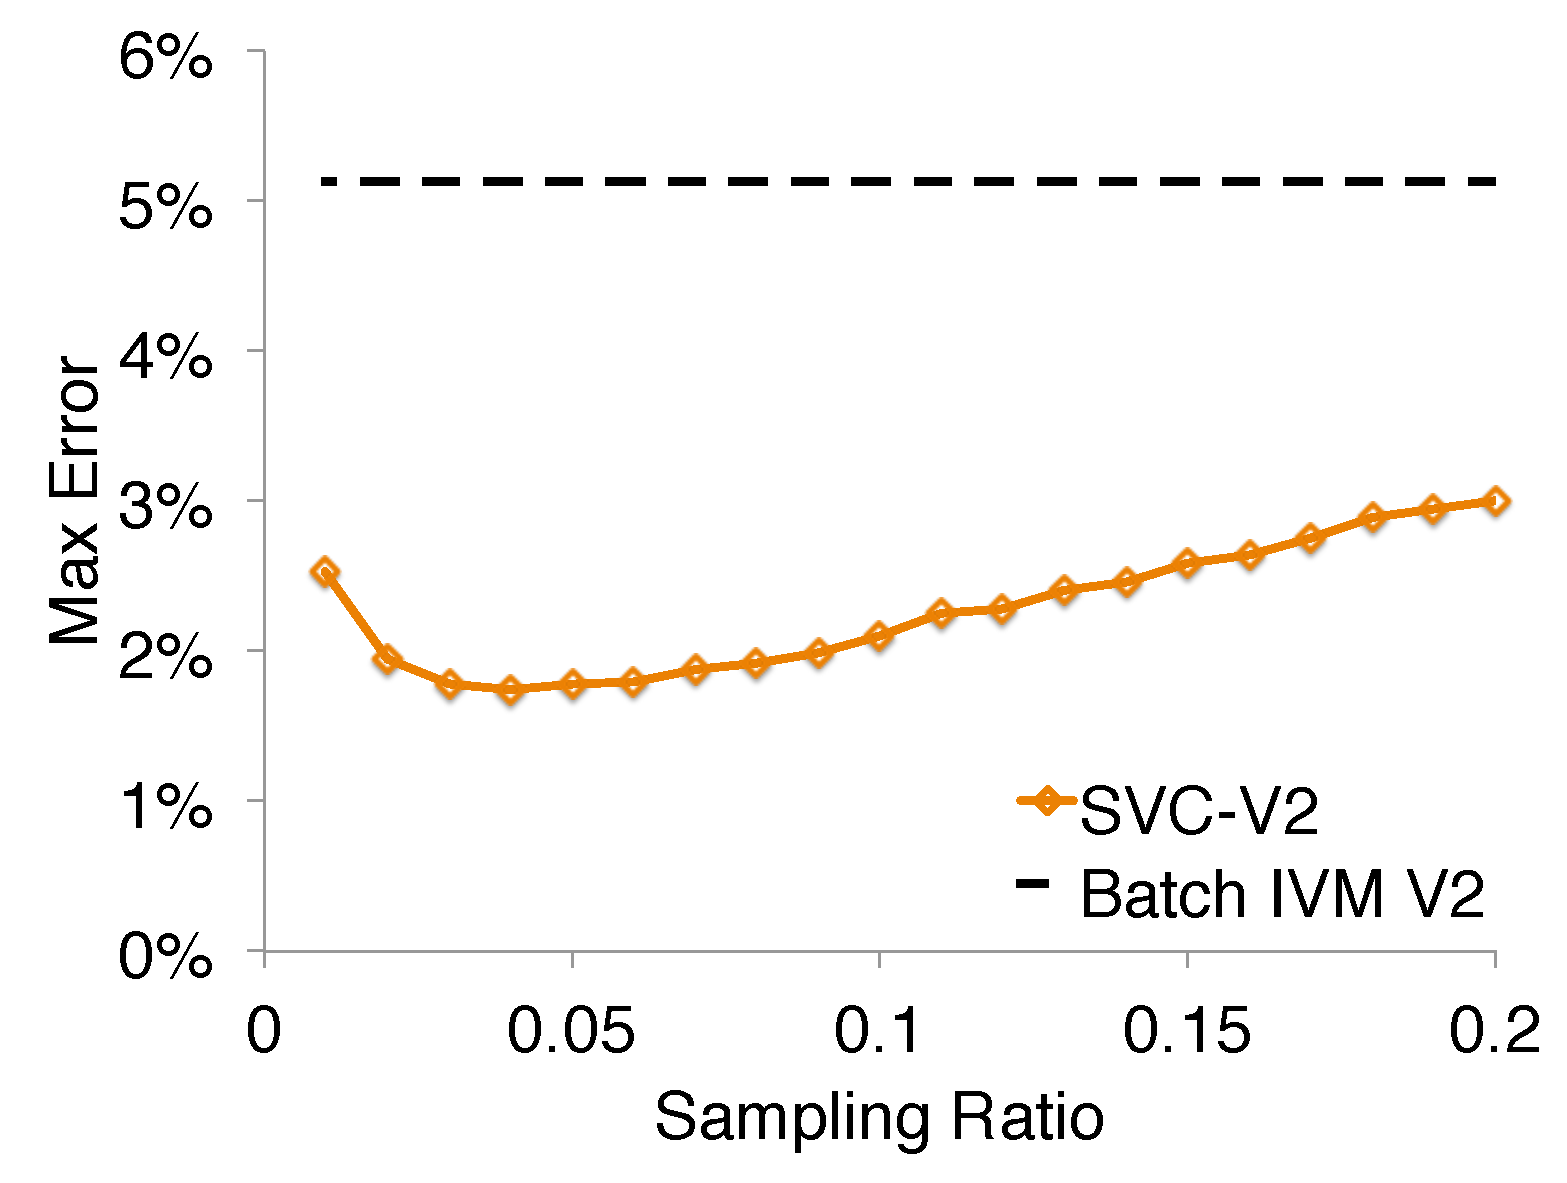
\includegraphics[scale=0.14]{exp/con_5.pdf}
 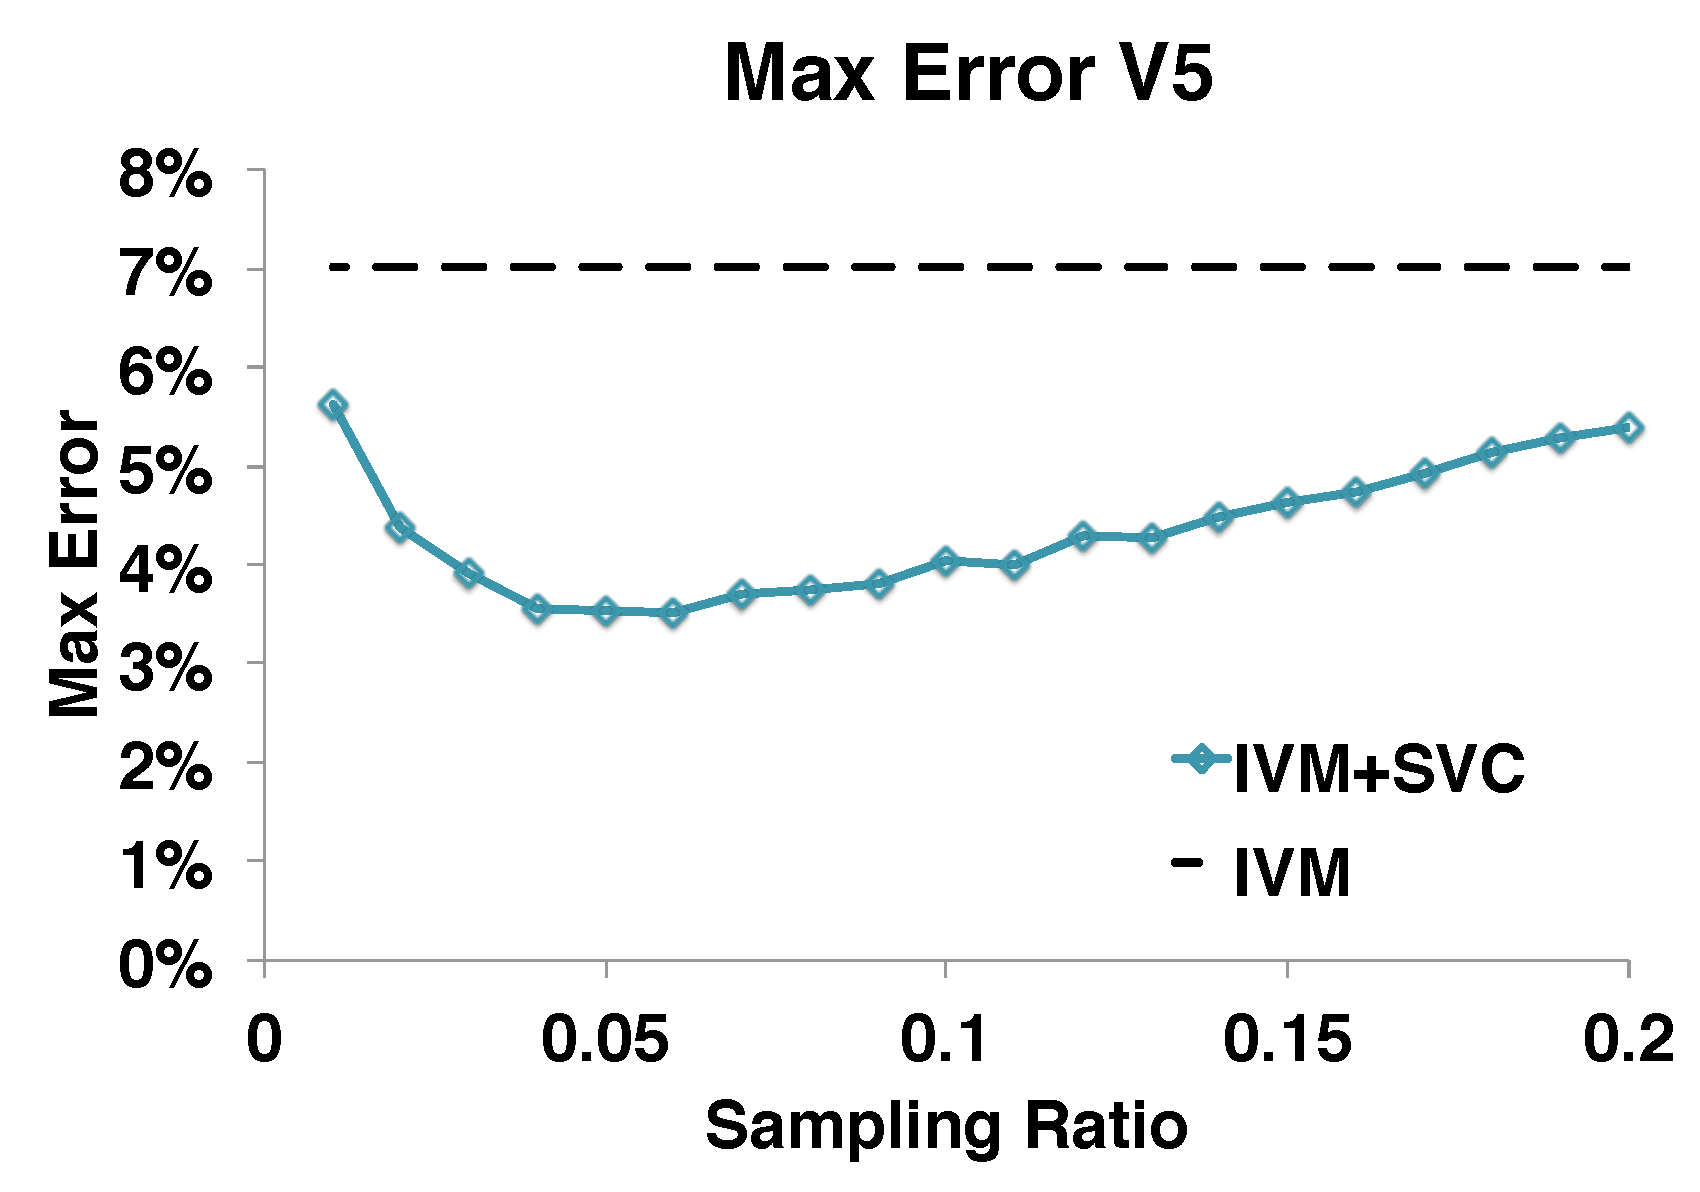
\includegraphics[scale=0.14]{exp/con_6.pdf}
 \caption{For a fixed throughput, SVC+Periodic Maintenance gives more accurate results for V2 and V5. \label{conv-4}} 
\end{figure}

\begin{figure}[t]
\centering
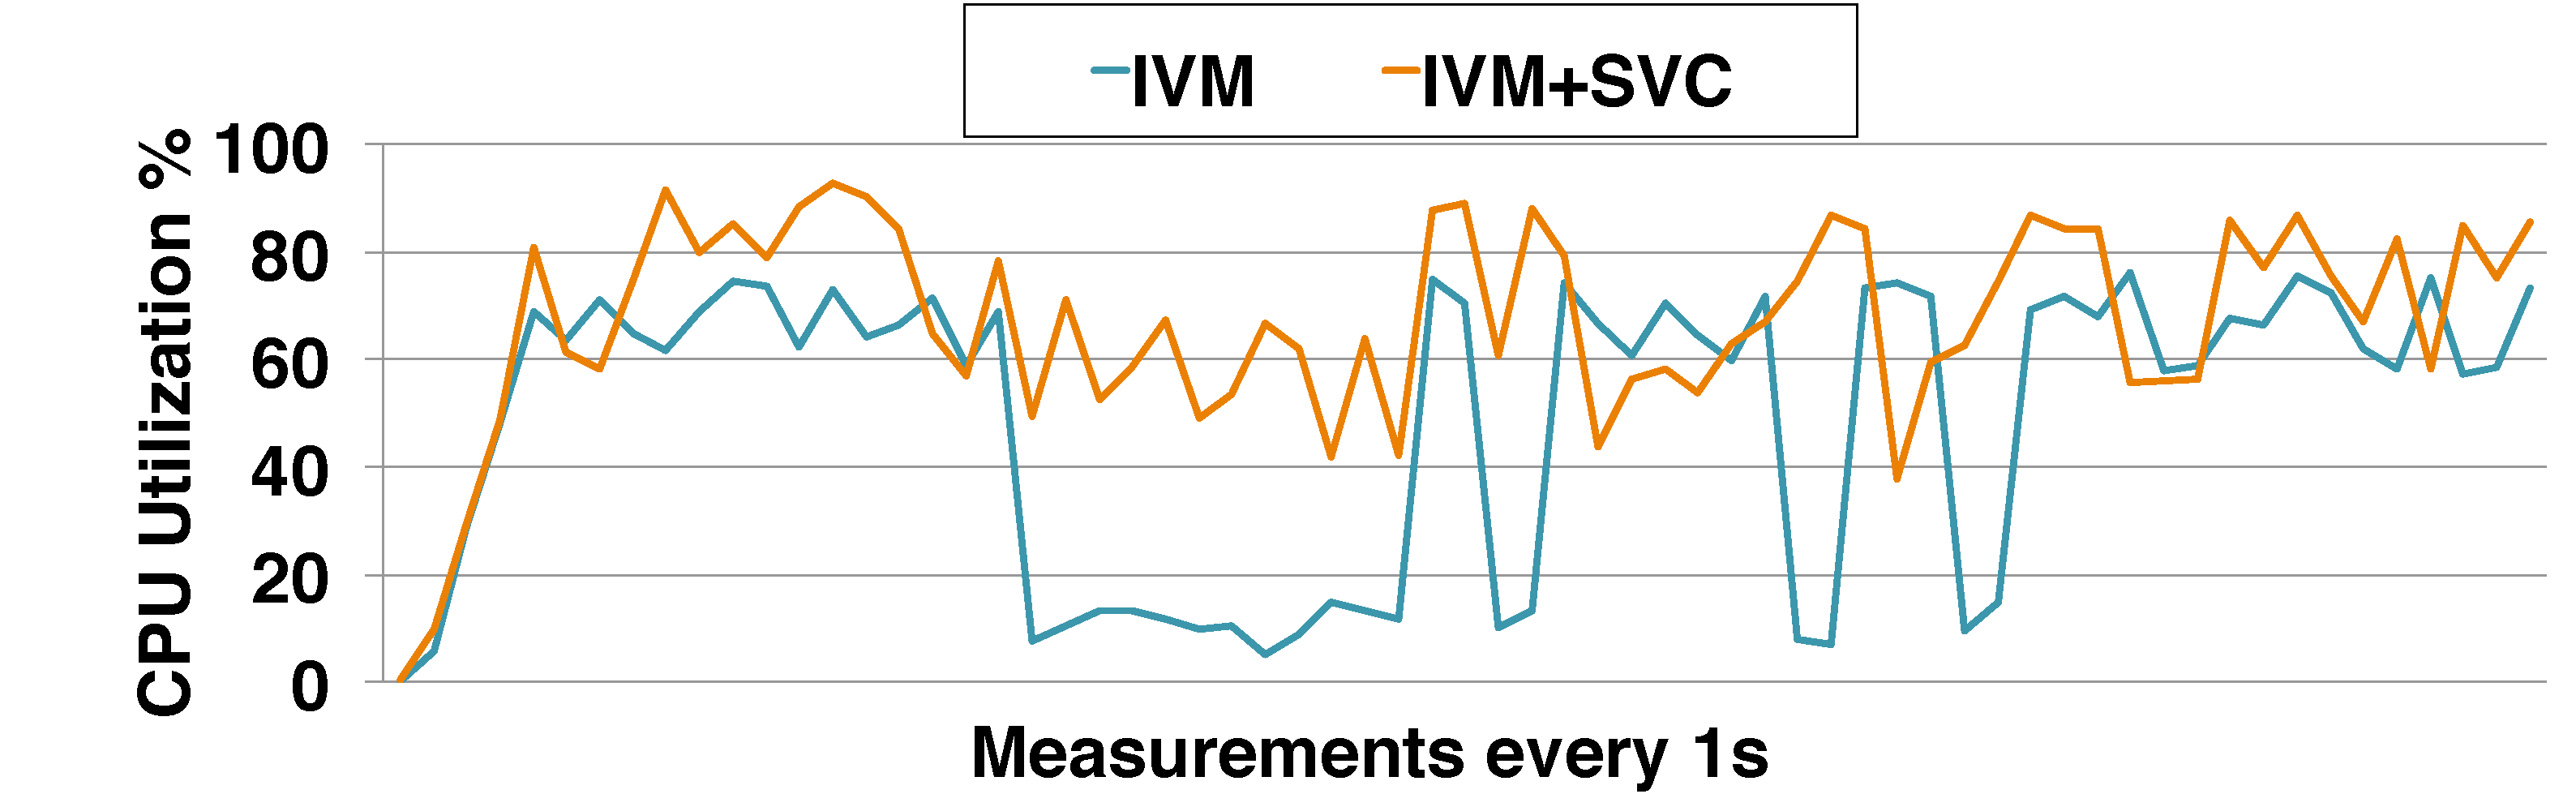
\includegraphics[width=\columnwidth]{exp/con_7.pdf}
 \caption{SVC better utilizes idle times in the cluster by maintaining the sample.\label{conv-5}} 
\end{figure}
To give some intuition on why SVC gives more accurate results, in Figure \ref{conv-5}, we plot the average CPU utilization of the cluster for both periodic IVM and SVC+periodic IVM. 
We find that SVC takes advantage of the idle times in the system; which are common during shuffle operations in a synchronous parallelism model.

In a way, these experiments present a worst-case application for SVC, yet it still gives improvements in terms of query accuracy.
In many typical deployments throughput demands are variable forcing maintenance periods to be longer, e.g., nightly.
The same way that SVC takes advantage of micro idle times during communication steps, it can provide large gains during controlled idle times when no maintenance is going on concurrently.

\subsection{Extended Proofs}

\subsection{Is Hashing Equivalent To RNG?}
In this work, we argue that hashing can be used for ``sampling" a relational expression.
However, from a complexity theory perspective, hashing is not equivalent to random number generation (RNG).
The existence of true one-way hash functions is a conjecture that would imply $P \ne NP$.
This conjecture is often taken as an assumption in Cryptography.
Of course, the ideal one-way hash functions required by the theory do not exist in practice. However, we find that existing hashes (e.g., linear hashes and SHA1) are sufficiently close to ideal that they can still take advantage of this theory. 
On the other hand, a SHA1 hash is nearly an order of magnitude slower but is much more uniform.
This assumption is called the Simple Uniform Hashing Assumption (SUHA) \cite{cormenintroduction}, and is widely used to analyze the performance of hash tables and hash partitioning.
There is an interesting tradeoff between the latency in computing a hash compared to its uniformity. For example, a linear hash stored procedure in MySQL is nearly as fast pseudorandom number generation that would be used in a TABLESAMPLE operator, however this hash exhibits some non-uniformity. 

\subsubsection{Hashing and Correspondence}
A benefit of deterministic hashing is that when applied in conjunction to the primary keys of a view, we get the Correspondence Property (Definition \ref{correspondence}) for free.
\begin{proposition}[Hashing Correspondence]
Suppose we have $S$ which is the stale view and $S'$ which is the up-to-date view.
Both these views have the same schema and a primary key $a$.
Let $\eta_{a, m}$ be our hash function that applies the hashing to the primary key $a$.
\[
\hat{S} = \eta_{a, m}(S)
\]
\[
\hat{S'} = \eta_{a, m}(S')
\]
Then, two samples $\hat{S'}$ and $\hat{S}$ correspond.
\end{proposition}
\begin{proof}
There are four conditions for correspondence:
\begin{itemize}
\item (1) Uniformity: $\widehat{S'}$ and $\widehat{S}$ are uniform random samples of $S'$ and $S$ respectively with a sampling ratio of $m$
\item (2) Removal of Superfluous Rows: $D = \{\forall s \in \widehat{S} \nexists s' \in S': s(u) = s'(u)\}$, $D \cap \widehat{S'} = \emptyset$ 
\item (3) Sampling of Missing Rows: $I = \{\forall s' \in \widehat{S'} \nexists s \in S: s(u) = s'(u)\}$, $\mathbb{E}(\mid I \cap \widehat{S'} \mid) = m\mid I \mid $ 
\item (4) Key Preservation for Updated Rows: For all $s\in \widehat{S}$ and not in $D$ or $I$, $s' \in \widehat{S}': s'(u) = s(u)$.
\end{itemize}
Uniformity is satisfied under by definition under SUHA (Simple Uniform Hashing Assumption).
Condition 2 is satisfied since if $r$ is deleted, then $r \not \in S'$ which implies that $r \not\in \hat{S'}$.
Condition 3 is just the converse of 2 so it is satisfied.
Condition 4 is satisfied since if $r$ is in $\hat{S}$ then it was sampled, and then since the primary key is consistent between $S$ and $S'$ it will also be sampled in $\hat{S'}$.
\end{proof}

\subsection{Theorem 1 Proof}
\begin{theorem}
Given a derived relation $R$, primary key $a$, and the sample $\eta_{a, m}(R)$.
Let $S$ be the sample created by applying $\eta_{a, m}$ without push down and 
$S'$ be the sample created by applying the push down rules to $\eta_{a, m}(R)$.
$S$ and $S'$ are identical samples with sampling ratio $m$.
\end{theorem}
\begin{proof}
We can prove this by induction.
The base case is where the expression tree is only one node, trivially making this true.
Then, we can induct considering one level of operators in the tree.
$\sigma, \cup, \cap, -$ clearly commute with hashing the key $a$ allowing for push down.
$\Pi$ commutes only if $a$ is in the projection.
For $\bowtie$, a sampling operator on $Q$ can be pushed down if $a$ is in either $k_r$ or $k_s$, or if there is a constraint that links $k_r$ to $k_s$.
There are two cases in which this happens a foreign-key relationship or an equality join on the same key.
For group by aggregates, if $a$ is in the group clause (i.e., it is in the aggregate) then a hash of the operand filters all rows that have $a$ which is sufficient to materialize the derived row.
It is provably NP-Hard to pushdown through a nested group by aggregate such as:
\begin{lstlisting}
SELECT c, count(1)
FROM ( 
       SELECT videoId, sum(1) as c FROM Log 
       GROUP BY videoId
     )
GROUP BY c
\end{lstlisting}
by reduction to a SUBSET-SUM problem.
\end{proof}

\subsection{More about the Hash Operator}
We defined a concept of tuple-lineage with primary keys.
However, a curious property of the deterministic hashing technique is that we can actually hash any attribute while retain the important statistical properties.
This is because a uniformly random sample of any attribute (possibly not unique) still includes every individual row with the same probability.  
A consequence of this is that we can push down the hashing operator through arbitrary equality joins (not just many-to-one) by hashing the join key.

We defer further exploration of this property to future work as it introduces new tradeoffs.
For example, sampling on a non-unique key, while unbiased in expectation, has higher variance in the size of the sample.
Happening to hash a large group may lead to decreased performance. 

Suppose our keys are duplicated $\mu_k$ times on average with variance $\sigma_k^2$, then the variance of the
sample size is for sampling fraction $m$:
\[m(1-m)\mu_k^2+(1-m)\sigma_k^2\]
This equation is derived from the formula for the variance of a mixture distribution.
In this setting, our sampling would have to consider this variance against the benefits of pushing the hash operator further down the query tree. 

\subsection{Experimental Details}

\subsubsection{Join View TPCD Queries}
In our first experiment, we materialize the join of lineitem and orders.
We treat the TPCD queries as queries on the view, and we selected 12 out of the 22 to include in our experiments.
The other 10 queries did not make use of the join.

\subsubsection{Conviva Views}
In this workload, there were annotated summary statistics queries, and we filtered for the most common types.
While, we cannot give the details of the queries, we can present some of the high-level characteristics of 8 summary-statistics type views. 
\begin{itemize} 
\item \textbf{V1.} Counts of various error types grouped by resources, users, date
\item \textbf{V2.} Sum of bytes transferred grouped by resource, users, date
\item \textbf{V3.} Counts of visits grouped by an expression of resource tags, users, date.
\item \textbf{V4.} Nested query that groups users from similar regions/service providers together then aggregates statistics
\item \textbf{V5.} Nested query that groups users from similar regions/service providers together then aggregates error types
\item \textbf{V6.} Union query that is filtered on a subset of resources and aggregates visits and bytes transferred
\item \textbf{V7.} Aggregate network statistics group by resources, users, date with many aggregates.
\item \textbf{V8.} Aggregate visit statistics group by resources, users, date with many aggregates.
\end{itemize}

\subsubsection{Data Cube Specification}
We defined the base cube as a materialized view:
\begin{lstlisting}
select
  sum(l_extendedprice * (1 - l_discount)) as revenue,
  c_custkey, n_nationkey,
  r_regionkey, L_PARTKEY
from
  lineitem, orders,
  customer, nation,
  region
where
  l_orderkey = o_orderkey and
  O_CUSTKEY = c_custkey and
  c_nationkey = n_nationkey and
  N_REGIONKEY = r_regionkey

group by
  c_custkey, n_nationkey, 
  r_regionkey, L_PARTKEY
\end{lstlisting}

Each of queries was an aggregate over subsets of the dimensions of the cube, 
with a \sumfunc over the revenue column.
\begin{itemize}
\item Q1. all
\item Q2. c\_custkey
\item Q3. n\_nationkey
\item Q4. r\_regionkey
\item Q5. l\_partkey
\item Q6. c\_custkey,n\_nationkey
\item Q7. c\_custkey,r\_regionkey
\item Q8. c\_custkey,l\_partkey
\item Q9. n\_nationkey, r\_regionkey
\item Q10. n\_nationkey, l\_partkey
\item Q11. c\_custkey,n\_nationkey, r\_regionkey
\item Q12. c\_custkey,n\_nationkey,l\_partkey
\item Q13. n\_nationkey,r\_regionkey,l\_partkey
\end{itemize}

When we experimented with the median query, we changed the \sumfunc to a median of the revenues.

\subsubsection{Table Of TPCD Queries 2}
We denormalize the TPCD schema and treat each of the 22 queries as views on the denormalized schema.
In our experiments, we evaluate 10 of these with SVC. 
Here, we provide a table of the queries and reasons why a query was not suitable for our experiments.
The main reason a query was not used was because the cardinality of the result was small.
Since we sample from the view, if the result was small eg. < 10, it would not make sense to apply SVC.
Furthermore, in the TPCD specification the only tables that are affected by updates are lineitem and orders; and queries that
do not depend on these tables do not change; thus there is no need for maintenance.

Listed below are excluded queries and reasons for their exclusion.
\begin{itemize}
\item Query 1. Result cardinality too small
\item Query 2. The query was static
\item Query 6. Result cardinality too small
\item Query 7. Result cardinality too small
\item Query 8. Result cardinality too small
\item Query 11. The query was static 
\item Query 12. Result cardinality too small
\item Query 14. Result cardinality too small
\item Query 15. The query contains an inner query, which we treat as a view.
\item Query 16. The query was static 
\item Query 17. Result cardinality too small
\item Query 19. Result cardinality too small
\item Query 20. Result cardinality too small
\end{itemize}


